\documentclass[12pt,fleqn]{ltjsarticle}
\usepackage[top=15truemm,bottom=15truemm,left=10truemm,right=10truemm]{geometry}
\usepackage{luatexja-fontspec}
\usepackage[ipaex]{luatexja-preset}
\usepackage{amsmath, amssymb}
\usepackage{empheq}
\usepackage{color}
%\usepackage{ascmac}
\begin{document}
\newcommand{\red}[1]{\textcolor{red}{#1}}
\renewcommand{\labelenumi}{(\arabic{enumi})}

\section{静電容量の計算}
$Q=CV$:同じ$V$でも$C$が大きいほうが$Q$が大きくなる。

つまり、$C$が大きい→多くの$Q$を蓄えることができる。

\subsection{}

\begin{minipage}{.2\linewidth}
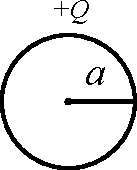
\includegraphics{14-1.pdf}
\end{minipage}
\hfill
\begin{minipage}{.8\linewidth}
\begin{align*}
V=\frac{Q}{4\pi \epsilon_0a}\rightarrow Q=4\pi\epsilon_0aV\\
(C=4\pi\epsilon_0a)
\end{align*}

$a$が大きいほど$C$が大きくなる。
\end{minipage}

\subsection{}

$C=\epsilon_0 \frac Sd$となる。(既習)

\subsection{同心球}

$a<r<b$における電界は\\
\begin{align*}
4\pi r^2E=\frac {Q}{\epsilon_0}より、E=\frac{Q}{4\pi\epsilon_0r^2}
\end{align*}
($C<r$には電界がない)
\begin{align*}
V&=-\int^a_b \frac{Q}{4\pi\epsilon_0r^2}dr
=-\frac{Q}{4\pi\epsilon_0}\int^a_b r^{-2}dr\\
&=-\frac{Q}{4\pi\epsilon_0}[(-1)r^{-1}]^a_b
=\frac{Q}{4\pi\epsilon_0}(\frac 1a - \frac 1b)\\
\therefore Q&=\frac{4\pi\epsilon_0}{\frac 1a - \frac 1b}V\\
\therefore C&=\frac{4\pi\epsilon_0}{\frac 1a - \frac 1b}
=\frac{4\pi\epsilon_0ab}{b-a}
\end{align*}
\begin{itemize}
\item $C$は無関係
\item $b\rightarrow \inf$とすると、例1に帰着する。
\end{itemize}

\subsection{同心円筒}

$a<r<b$における電界は、
\begin{align*}
&2\pi r\cdot lE=\frac{\lambda l}{\epsilon_0}
\therefore E=\frac{\lambda}{2\pi\epsilon_0r}\\
V&=-\int^a_b\frac{\lambda}{2\pi\epsilon_0r}dr
=-\frac{\lambda}{2\pi\epsilon_0}\int^a_b r^{-1}dr\\
&=\frac{\lambda}{2\pi\epsilon_0}[\ln r]^a_b
=-\frac{\lambda}{2\pi\epsilon_0}\ln \frac ab\\
&=\frac{\lambda}{2\pi\epsilon_0}\ln ba\\
\therefore \lambda&=\frac{2\pi\epsilon_0}{\ln{b/a}}V\\
&\left(C=\frac{2\pi\epsilon_0}{\ln{b/a}}\right)
\end{align*}
\subsection{送電線}

$x$の場所における電界を求める。
\begin{align*}
&Aによる電界:\frac{\lambda}{2\pi\epsilon_0x}\\
&Bによる電界:\frac{\lambda}{2\pi\epsilon_0(d-x)}
\end{align*}

($\lambda$が均一に分布していると仮定する。ただし$r<<d$)

\newcommand{\el}{\frac{\lambda}{2\pi\epsilon_0}}

\begin{align*}
\therefore E&=\el
\left(\frac 1x + \frac 1{d-x}\right)\\
V&=-\int^r_{d-r}Edx=\int^{d-r}_rEdx
=\int^{d-r}_r\el(\frac1x+\frac1{d-x})dx\\
&=\el[\ln x - \ln{(d-x)}]^{d-r}_r
=\el\left[\ln\frac x{d-x}\right]^{d-r}_r\\
&=\frac{\lambda}{\pi\epsilon_0}\ln\frac{d-r}r
\simeq \lambda\frac{\ln\frac dr}{\pi\epsilon_0}(d>>r)\\
\therefore \lambda&=\frac{\pi\epsilon_0}{\ln{d/r}}V
\therefore C=\frac{\pi\epsilon_0}{\ln{d/r}}l(F)
\end{align*}

\subsection{2つの導体球}
\renewcommand{\el}[1]{\frac Q{4\pi\epsilon_0 #1}}

\begin{align*}
Aによる電界:\el{x^2}\\
Bによる電界:\el{(d-x)^2}
\end{align*}
\begin{align*}
\therefore E&=\el{}\left(\frac 1{x^2} + \frac 1{(d-x)^2}\right)\\
V&=\int^{d-r}_r \el{}\left(\frac 1{x^2} + \frac 1{(d-x)^2}\right)dx\\
&=\el{}\left[\frac 1x + \frac 1{d-x}\right]^{d-r}_r\\
&=\el{}\left\{(-\frac1{d-r}+\frac1r)-(-\frac1r+\frac1{d-r})\right\}\\
&=\el{}\left(\frac2r-\frac2{d-r}\right)
=2\cdot\el{}\left(\frac1r-\frac1{d-r}\right)\\
&\sim \frac Q{2\pi\epsilon_0}(\frac1r - \frac 1d)\\
Q&\sim \frac{2\pi\epsilon_0}{\frac1r - \frac 1d}V
\therefore C\sim \frac{2\pi\epsilon_0rd}{d-r}(F)
\end{align*}
\end{document}
